\section{Experiments}
\label{sec:experiments}

\subsection{Overview}
\label{sub:overview}

To analyze the performance of our parallel \ac{GP} algorithm, we used synthetic datasets.
We assume that the precision of the noise, $\beta^{-1}$, was known to simplify the
computation of the log-likelihood gradients.  We used two datasets: one with 10,000
training points and one with 100,000 training points.  Datasets of this size {\bf require}
the use of a sparse kernel because otherwise it is unreasonable to store
$\mat{C}_N$ in memory.  Due to deadline constraints and waiting times on the CAEN CAC
cluster queue, we use only 1D features, so that the Type 1 and Type 2 kernels are
equivalent.

We do not report the \ac{MSE} of our dataset because the focus of our project is on
computation time.  The accuracy of the \ac{GP} for testing datasets under a variety of
noise conditions has already been studied extensively, including for sparse kernels.
Since we are not doing any approximations to the \ac{GP}, we stick primarily to timing
results.  Those who are curious about the qualitative results of our implementation should
refer to Figure~\ref{fig:learn} as verification that our code computes the GP correctly.

\subsection{Results and Discussion}
\label{sub:results}

Starting with the computation of the covariance matrix $\mat{C}_N$ from
Equation~\ref{eqn:cov}, we see some surprising results.  In particular, we observe that
the speedup of the algorithm is super-linear, as shown in Figure~\ref{fig:cov}.  This is
not expected because each element of the covariance matrix can be computed entirely
independently from each other.  This implies the algorithm should achieve near-perfect
linear speedup.  Though we have not found the root cause of the super-linear speedup, we
suspect that the internal behavior of the \ac{PETSc} library is causing unusually slow
execution time when computing $\mat{C}_N$ when $p$ is small.  In other words, the parallel
execution time is probably accurate, but the serial time is slower than it should be.
However, this is not cause for much concern because computing $\mat{C}_N$ is not the
bottleneck of sparse \ac{GP} regression.  The full list of execution times is shown in
Tables~\ref{tab:Ksmall} and \ref{tab:Kbig} for the 10,000 and 100,000-point datasets,
respectively.

Next, we analyzed the performance of each gradient descent step that involves computing
Equation~\ref{eqn:learn}.  For both of the synthetic datasets, we compute the speedup and
efficiency as $p$, the number of \acp{PE}, varies from 1 (serial) to 36 (the maximum
number our EECS 587 accounts were allocated).  For the 10,000-length dataset, we also
consider the effect of the sparsity of $\mat{C}_N$ on the speedup and efficiency.  The
sparsity of $\mat{C}_N$ can be tuned by varying $l_i$.

The timing results of computing Equation~\ref{eqn:learn} show that the efficiency of the
algorithm depends on both the size and sparsity of the covariance matrix, $\mat{C}_N$,
computed in Equation~\ref{eqn:cov}.  If $\mat{C}_N$ is small, containing only 10,000
columns, and very sparse with less than one percent nonzero entries, our algorithm
achieves fairly low efficiency.  However, as the matrix becomes more dense with 11.6\%
nonzero entries, the efficiency becomes close to linear.  These results are shown in the
speedup and efficiency curves from Figure~\ref{fig:grad} and the timing results tables are
shown in Tables~\ref{tab:grad} and ~\ref{tab:gradBig}.

\begin{table}
  \begin{center}
    % BEGIN RECEIVE ORGTBL Ksmall
    \begin{tabular}{|r|c|c|c|}
      \hline
      p & Seconds to compute & Speedup & Efficiency \\
      & Equation (\ref{eqn:cov}) &  &  \\
      \hline
      1 & 8.30 / 214.8 / 2500.19 & -- & -- \\
      4 & 1.02 / 16.63 / 1146.26 & 8.15 / 12.92 / 2.18 & 2.04 / 3.23 / 0.55 \\
      9 & 0.39 / 4.27 / 369.1 & 21.12 / 50.33 / 6.77 & 2.35 / 5.59 / 0.75 \\
      16 & 0.22 / 1.38 / 128.3 & 36.89 / 155.73 / 19.50 & 2.31 / 9.73 / 1.22 \\
      25 & 0.14 / 0.60 / 47.90 & 57.64 / 356.56 / 52.24 & 2.31 / 14.26 / 2.09 \\
      36 & 0.14 / 0.39 / 25.07 & 60.42 / 522.90 / 99.74 & 1.68 / 15.36 / 2.77 \\
      \hline
    \end{tabular}
    % END RECEIVE ORGTBL Ksmall
    \caption {{\small Time to compute the covariance matrix for the 10,000-point dataset.
        The results are shown for different amounts of sparsity, from left to right: 0.1\%
        nonzero, 1.3\% nonzero, and 11.6\% nonzero.  }}
    \label{tab:Ksmall}
  \end{center}
\end{table}

\begin{comment}
  #+ORGTBL: SEND Ksmall orgtbl-to-latex :splice nil :skip 0
  |----+--------------------------+------------------------+---------------------|
  |  p | Seconds to compute       | Speedup                | Efficiency          |
  |    | Equation (\ref{eqn:cov}) |                        |                     |
  |----+--------------------------+------------------------+---------------------|
  |  1 | 8.30 / 214.8 / 2500.19   | --                     | --                  |
  |  4 | 1.02 / 16.63 / 1146.26   | 8.15 / 12.92 / 2.18    | 2.04 / 3.23 / 0.55  |
  |  9 | 0.39 / 4.27 / 369.1      | 21.12 / 50.33 / 6.77   | 2.35 / 5.59 / 0.75  |
  | 16 | 0.22 / 1.38 / 128.3      | 36.89 / 155.73 / 19.50 | 2.31 / 9.73 / 1.22  |
  | 25 | 0.14 / 0.60 / 47.90      | 57.64 / 356.56 / 52.24 | 2.31 / 14.26 / 2.09 |
  | 36 | 0.14 / 0.39 / 25.07      | 60.42 / 522.90 / 99.74 | 1.68 / 15.36 / 2.77 |
  |----+--------------------------+------------------------+---------------------|
\end{comment}

\begin{table}
  \begin{center}
    % BEGIN RECEIVE ORGTBL Kbig
    \begin{tabular}{|r|c|c|c|}
      \hline
      p & Seconds to compute & Speedup & Efficiency \\
      & Equation (\ref{eqn:cov}) &  &  \\
      \hline
      1 & 566.56 & -- & -- \\
      4 & 98.43 & 5.76 & 1.44 \\
      9 & 42.94 & 13.19 & 1.47 \\
      16 & 23.34 & 24.27 & 1.52 \\
      25 & 13.79 & 41.08 & 1.64 \\
      36 & 9.51 & 59.58 & 1.65 \\
      \hline
    \end{tabular}
    % END RECEIVE ORGTBL Kbig
    \caption {{\small Time to compute the covariance matrix for the 100,000-point dataset.
      }}
    \label{tab:Kbig}
  \end{center}
\end{table}
\begin{comment}
  #+ORGTBL: SEND Kbig orgtbl-to-latex :splice nil :skip 0
  |----+--------------------------+---------+------------|
  |  p |       Seconds to compute | Speedup | Efficiency |
  |    | Equation (\ref{eqn:cov}) |         |            |
  |----+--------------------------+---------+------------|
  |  1 |                   566.56 |      -- |         -- |
  |  4 |                    98.43 |    5.76 |       1.44 |
  |  9 |                    42.94 |   13.19 |       1.47 |
  | 16 |                    23.34 |   24.27 |       1.52 |
  | 25 |                    13.79 |   41.08 |       1.64 |
  | 36 |                     9.51 |   59.58 |       1.65 |
  |----+--------------------------+---------+------------|
\end{comment}

\begin {table}
  \begin{center}
    % BEGIN RECEIVE ORGTBL gradtiming
    \begin{tabular}{|r|c|c|c|}
      \hline
      p & Seconds to compute & Speedup & Efficiency \\
      & Equation (\ref{eqn:learn}) &  &  \\
      \hline
      1 & 187.15 / 2739.8 / 22353.0 & -- & -- \\
      2 & 108.3 / 1436.3 / 12010.3 & 1.73 / 1.91 / 1.86 & 0.86 / 0.95 / 0.93 \\
      3 & 74.4 / 1055.5 / 7584.2 & 2.51 / 2.60 / 2.95 & 0.83 / 0.86 / 0.98 \\
      4 & 57.4 / 840.4 / 5601.3 & 3.26 / 3.26 / 3.99 & 0.81 / 0.81 / 0.99 \\
      9 & 29.9 / 493.6 / 2817.1 & 6.26 / 5.55 / 7.93 & 0.70 / 0.62 / 0.88 \\
      16 & 32.8 / 384.8 / 1505.7 & 5.71 / 7.12 / 14.85 & 0.36 / 0.45 / 0.93 \\
      25 & 30.9 / 314.5 / 1050.4 & 6.06 / 8.71 / 21.28 & 0.24 / 0.35 / 0.85 \\
      36 & 40.8 / 279.6 / 775.6 & 4.59 / 9.80 / 28.82 & 0.12 / 0.27 / 0.80 \\
      \hline
    \end{tabular}
    % END RECEIVE ORGTBL gradtiming
    \caption {{\small Time to compute the log-likelihood gradient from
        Equation~\ref{eqn:learn} using the 10,000-point dataset.  The results are shown
        for different amounts of sparsity, from left to right: 0.1\% nonzero, 1.3\%
        nonzero, and 11.6\% nonzero.  }}
    \label{tab:grad}
  \end{center}
\end {table}
\begin{comment}
  #+ORGTBL: SEND gradtiming orgtbl-to-latex :splice nil :skip 0
  |----+----------------------------+---------------------+--------------------|
  |  p | Seconds to compute         | Speedup             | Efficiency         |
  |    | Equation (\ref{eqn:learn}) |                     |                    |
  |----+----------------------------+---------------------+--------------------|
  |  1 | 187.15 / 2739.8 / 22353.0  | --                  | --                 |
  |  2 | 108.3 / 1436.3 / 12010.3   | 1.73 / 1.91 / 1.86  | 0.86 / 0.95 / 0.93 |
  |  3 | 74.4 / 1055.5 / 7584.2     | 2.51 / 2.60 / 2.95  | 0.83 / 0.86 / 0.98 |
  |  4 | 57.4 / 840.4 / 5601.3      | 3.26 / 3.26 / 3.99  | 0.81 / 0.81 / 0.99 |
  |  9 | 29.9 / 493.6 / 2817.1      | 6.26 / 5.55 / 7.93  | 0.70 / 0.62 / 0.88 |
  | 16 | 32.8 / 384.8 / 1505.7      | 5.71 / 7.12 / 14.85 | 0.36 / 0.45 / 0.93 |
  | 25 | 30.9 / 314.5 / 1050.4      | 6.06 / 8.71 / 21.28 | 0.24 / 0.35 / 0.85 |
  | 36 | 40.8 / 279.6 / 775.6       | 4.59 / 9.80 / 28.82 | 0.12 / 0.27 / 0.80 |
  |----+----------------------------+---------------------+--------------------|
\end{comment}

\begin {table}
  \begin{center}
    % BEGIN RECEIVE ORGTBL gradtimingbig
    \begin{tabular}{|r|c|c|c|}
      \hline
      p & Seconds to compute & Speedup & Efficiency \\
      & Equation (\ref{eqn:learn}) &  &  \\
      \hline
      1 & 26015.1 & -- & -- \\
      2 & 13883.3 & 1.87 & 0.94 \\
      3 & 9190.7 & 2.83 & 0.94 \\
      4 & 6686.8 & 3.89 & 0.97 \\
      9 & 4058.7 & 6.40 & 0.71 \\
      16 & 1877.3 & 13.85 & 0.87 \\
      25 & 1111.6 & 23.4 & 0.94 \\
      36 & 887.1 & 29.3 & 0.81 \\
      \hline
    \end{tabular}
    % END RECEIVE ORGTBL gradtimingbig
    \caption {{\small Time to compute the log-likelihood gradient from
        Equation~\ref{eqn:learn} for the 100,000-point dataset.  Even though the matrix is
        very sparse with 0.05\% nonzero elements, we can achieve near-linear speedup,
        unlike the results from the 10,000-point dataset where the matrix had to be
        relatively dense to achieve good efficiency.}}
    \label{tab:gradBig}
  \end{center}
\end {table}

\begin{comment}
  #+ORGTBL: SEND gradtimingbig orgtbl-to-latex :splice nil :skip 0
  |----+----------------------------+---------+------------|
  |  p |         Seconds to compute | Speedup | Efficiency |
  |    | Equation (\ref{eqn:learn}) |         |            |
  |----+----------------------------+---------+------------|
  |  1 |                    26015.1 |      -- |         -- |
  |  2 |                    13883.3 |    1.87 |       0.94 |
  |  3 |                     9190.7 |    2.83 |       0.94 |
  |  4 |                     6686.8 |    3.89 |       0.97 |
  |  9 |                     4058.7 |    6.40 |       0.71 |
  | 16 |                     1877.3 |   13.85 |       0.87 |
  | 25 |                     1111.6 |    23.4 |       0.94 |
  | 36 |                      887.1 |    29.3 |       0.81 |
  |----+----------------------------+---------+------------|
\end{comment}

\begin{figure}[t]
  \begin{center}
    \subfigure[Speedup (10,000 points)] {
      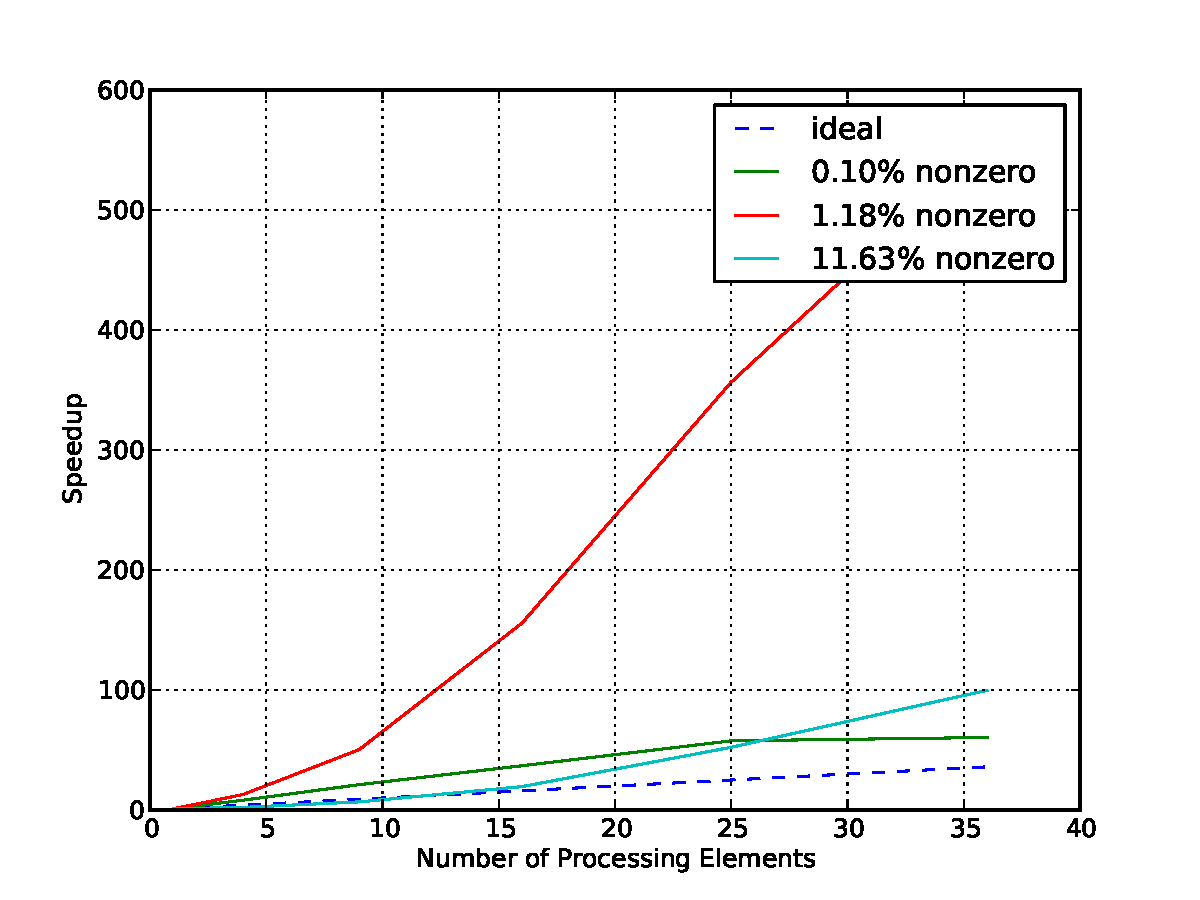
\includegraphics[width=0.46\textwidth]{figures/speedup_K_1e4}
      \label{fig:cov:s10k}}
    \subfigure[Speedup (100,000 points)] {
      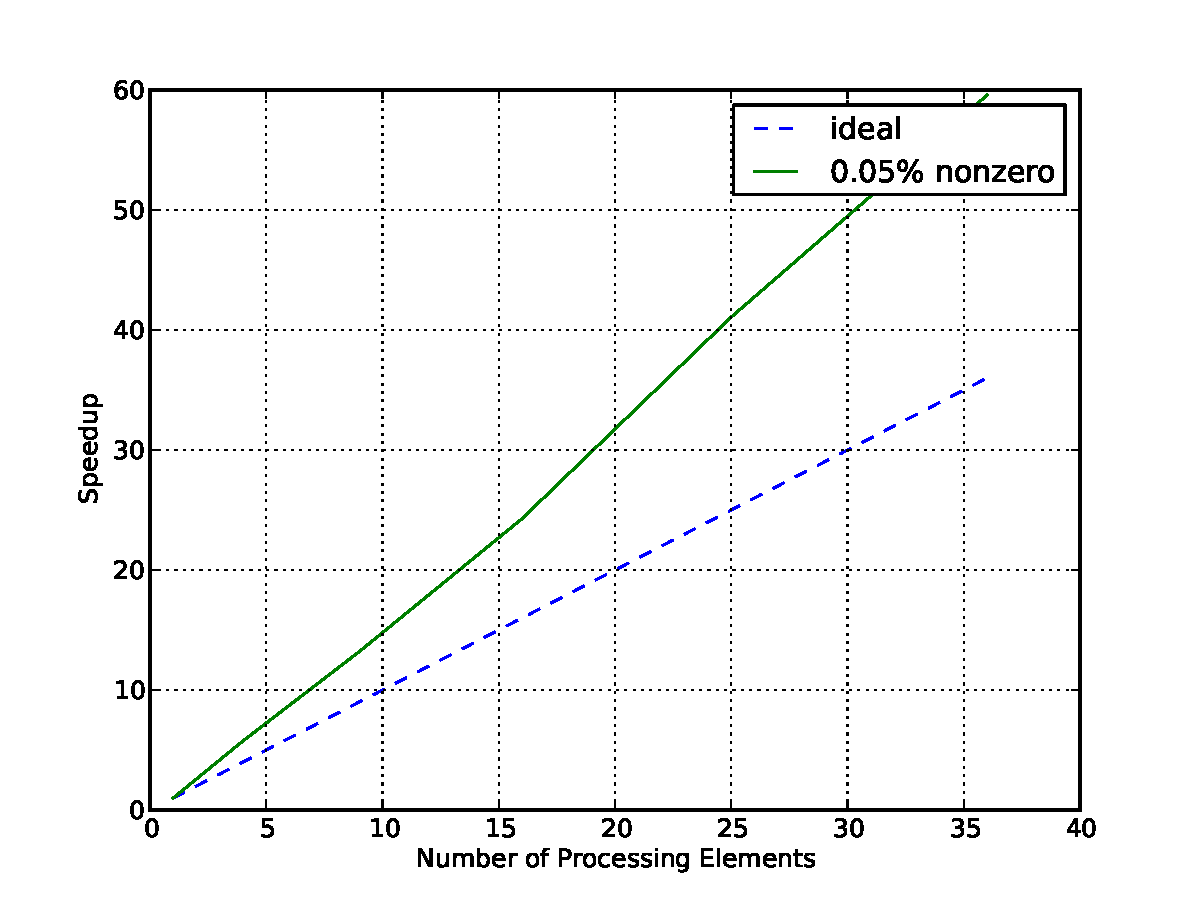
\includegraphics[width=0.46\textwidth]{figures/speedup_K_1e5}
      \label{fig:cov:s100k}}
    \subfigure[Efficiency (10,000 points)] {
      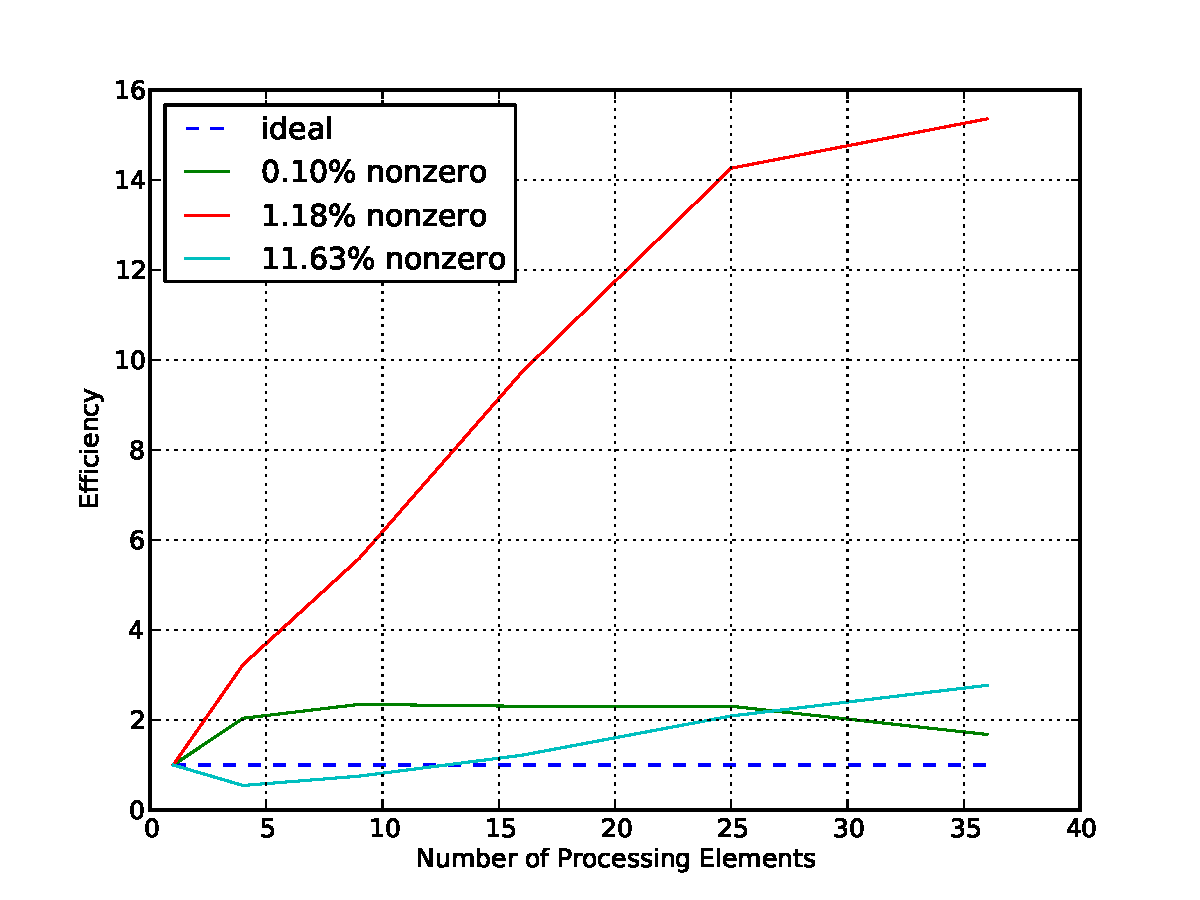
\includegraphics[width=0.46\textwidth]{figures/effic_K_1e4}
      \label{fig:cov:e10k}}
    \subfigure[Efficiency (100,000 points)] {
      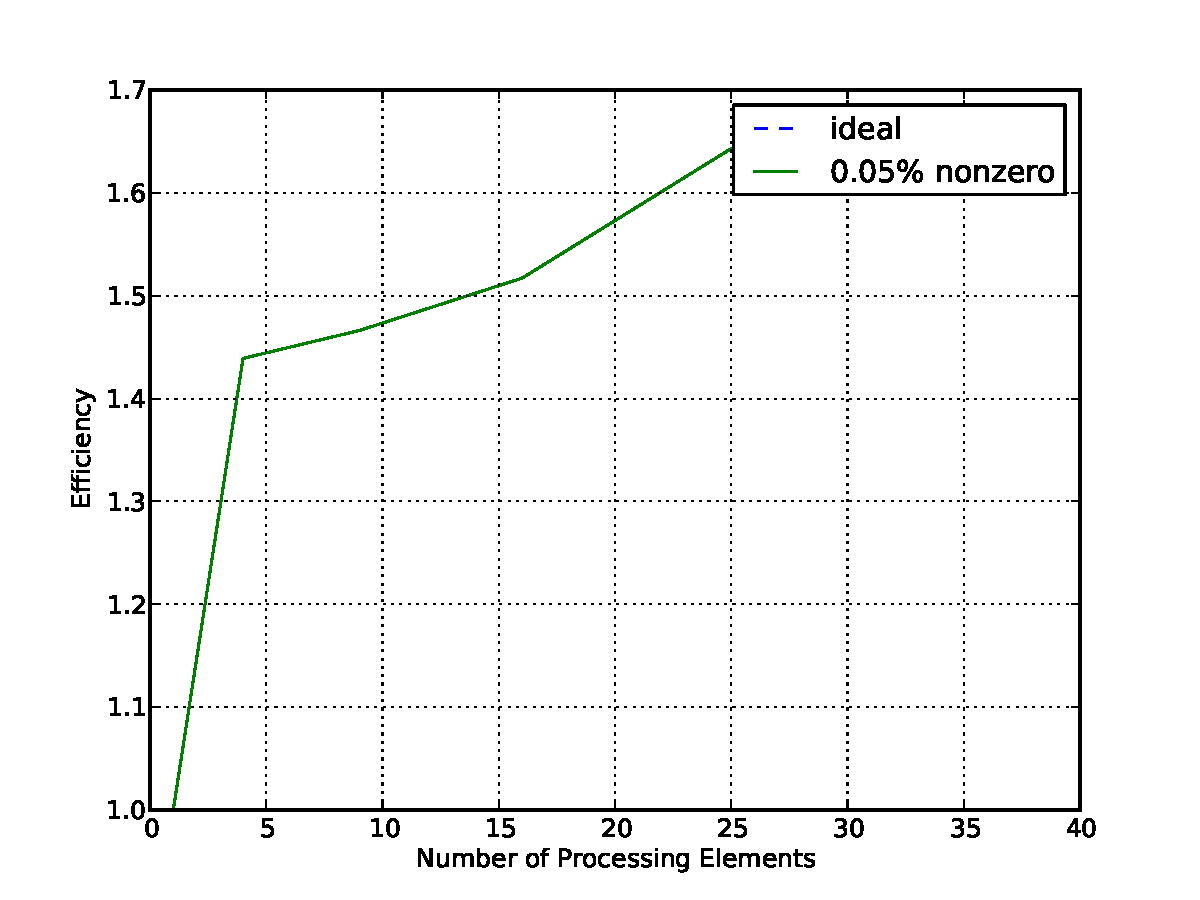
\includegraphics[width=0.46\textwidth]{figures/effic_K_1e5}
      \label{fig:cov:e100k}}
    \caption{{\small The performance results for computing Equation~\ref{eqn:cov}.  The
        green, red, and cyan lines denote the 0.10\% nonzero, 1.18\% nonzero, and 11.63\%
        nonzero cases, respectively.  Surprisingly, our implementation achieves super linear
        speedup, regardless of the matrix size or sparsity.  This is probably due to the
        way the PETSc library is implemented -- the \texttt{SetMatValues()} routine does
        some internal caching before actually applying the values, and we think this
        explains why the speedup and efficiency are higher than what is expected.  Because
        computing Equation~\ref{eqn:cov} should be nearly perfectly parallelizable, we
        expect near-exact linear speedup, neglecting the effects of any third-party
        packages. }}
    \label{fig:cov}
  \end{center}
\end{figure}

\begin{figure}[t]
  \begin{center}
    \subfigure[Speedup (10,000 points)] {
      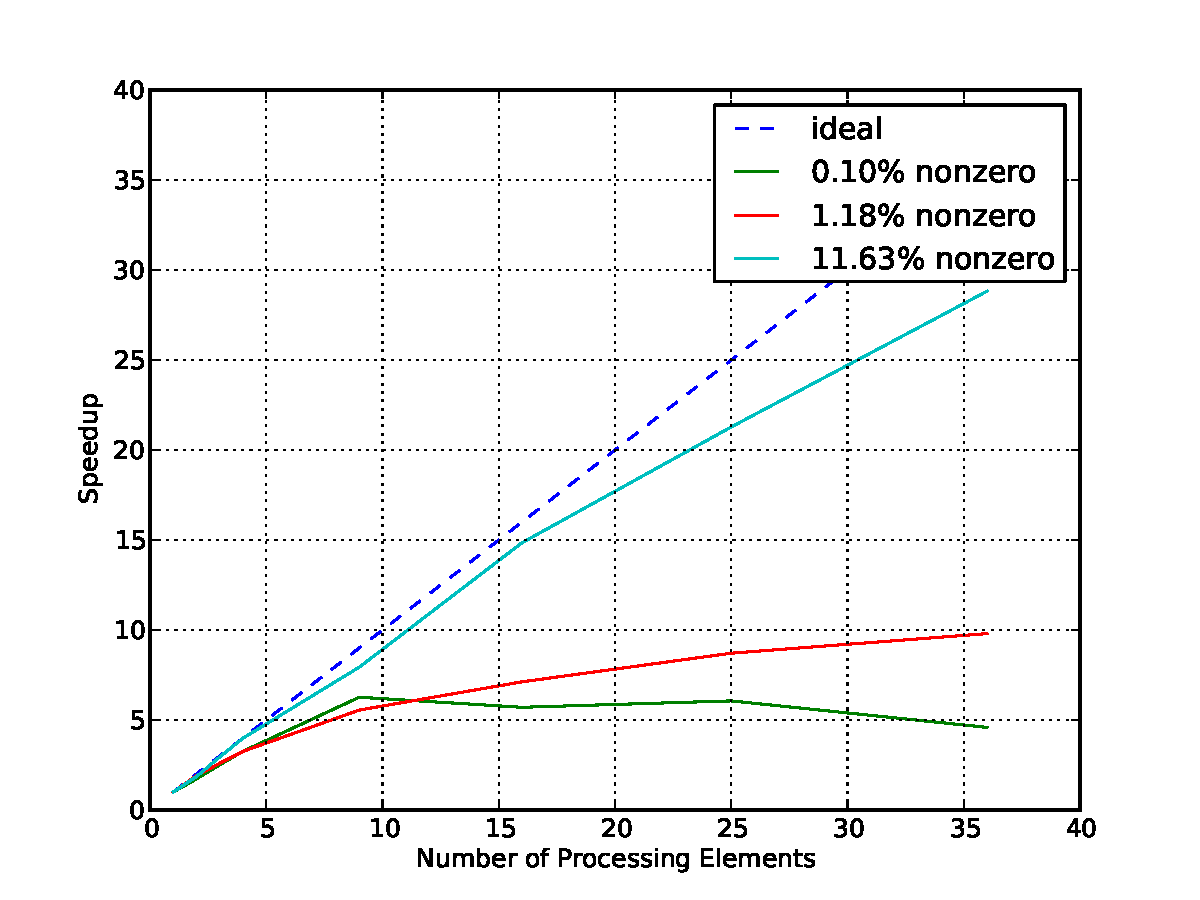
\includegraphics[width=0.46\textwidth]{figures/speedup_grad_1e4}
      \label{fig:grad:s10k}}
    \subfigure[Speedup (100,000 points)] {
      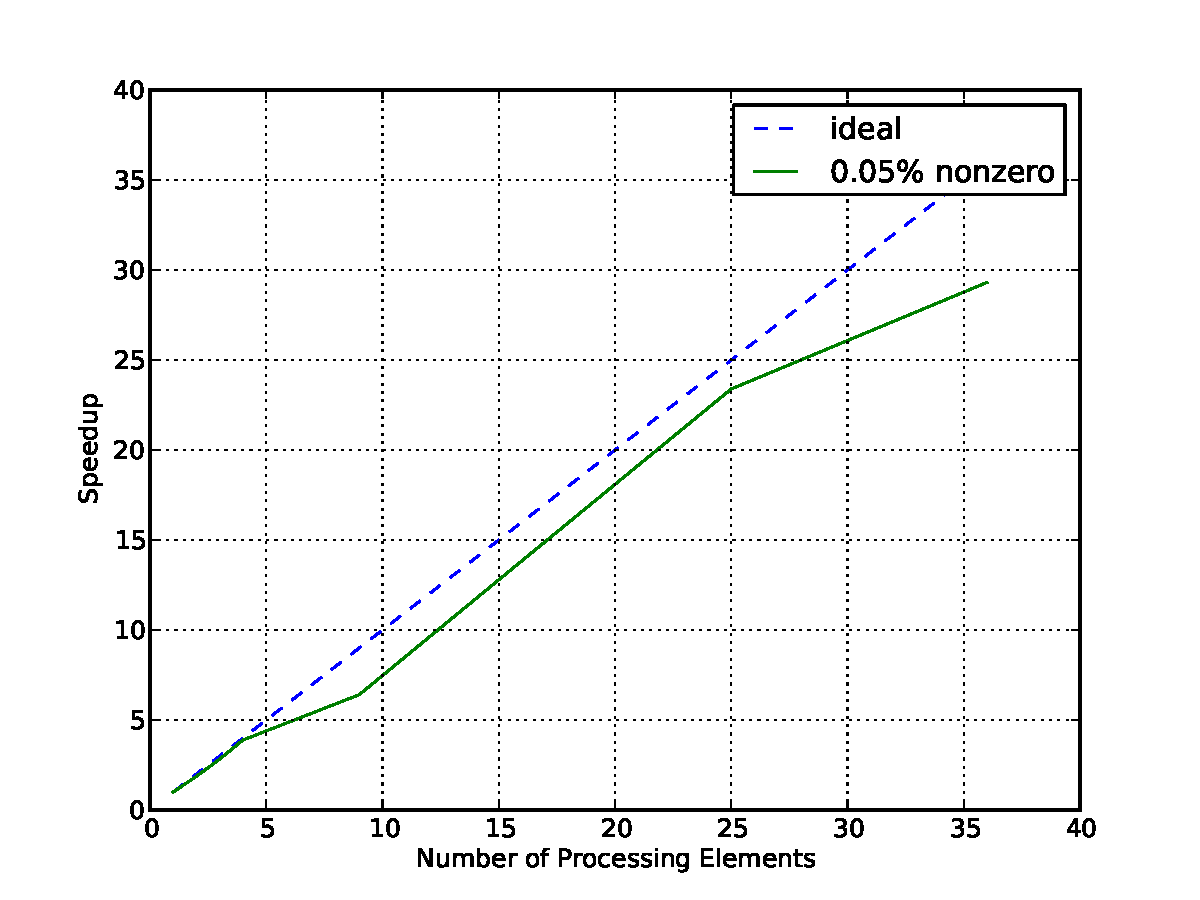
\includegraphics[width=0.46\textwidth]{figures/speedup_grad_1e5}
      \label{fig:grad:s100k}}
    \subfigure[Efficiency (10,000 points)] {
      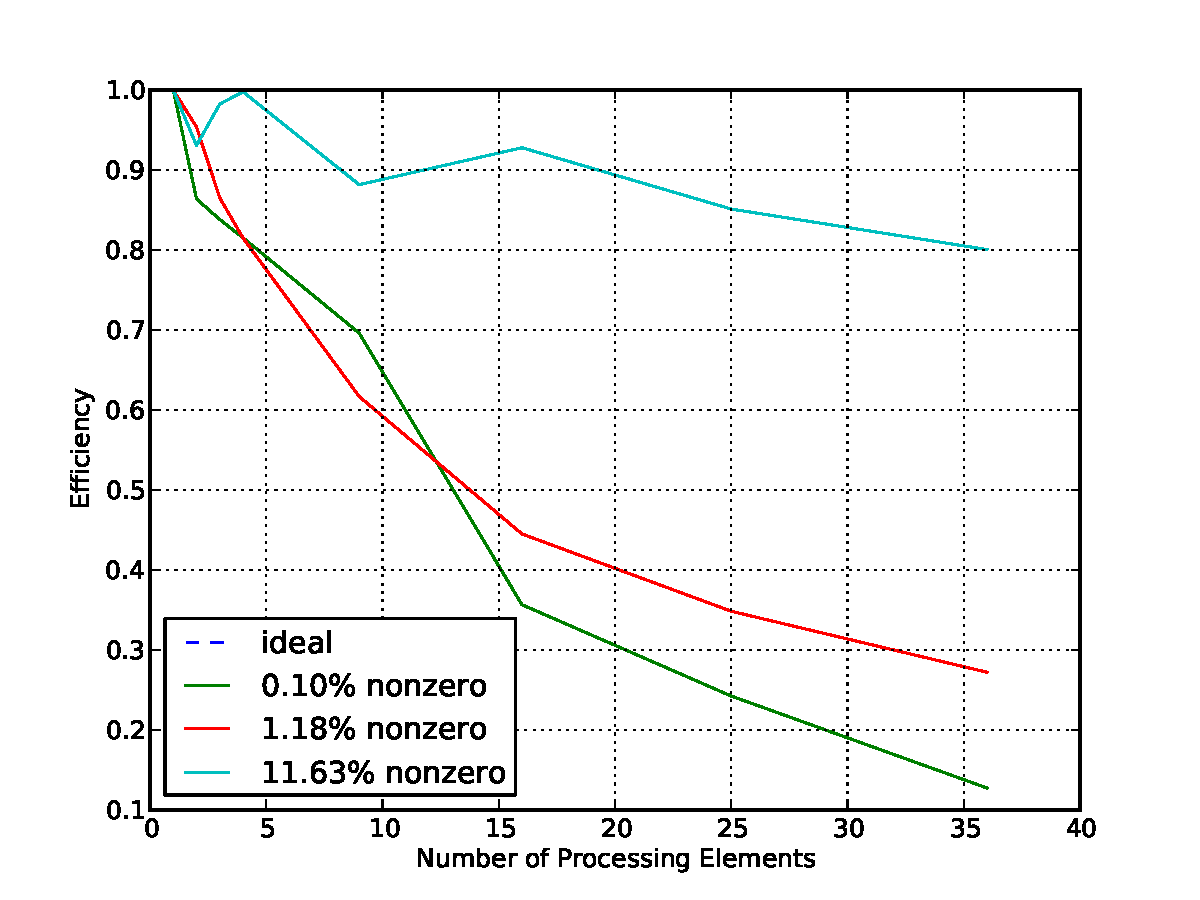
\includegraphics[width=0.46\textwidth]{figures/effic_grad_1e4}
      \label{fig:grad:e10k}}
    \subfigure[Efficiency (100,000 points)] {
      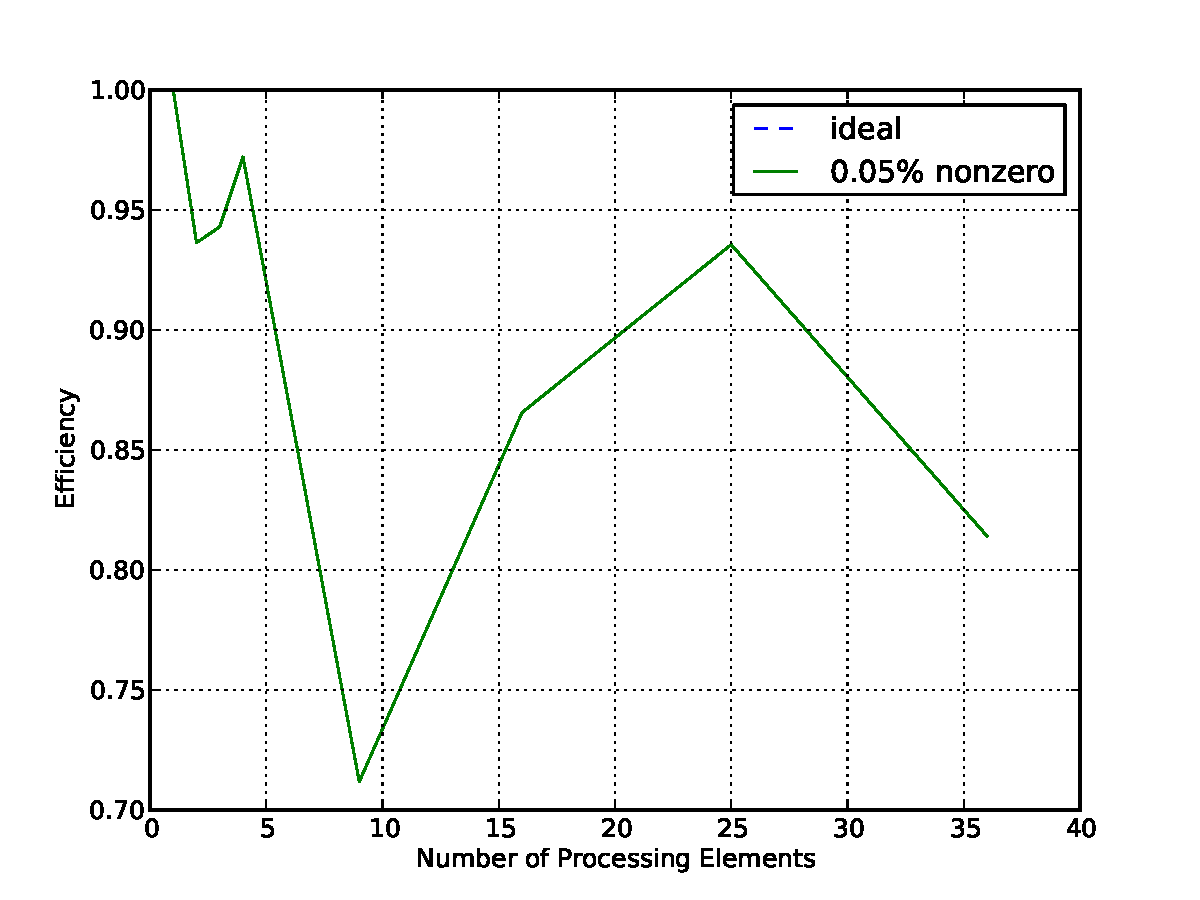
\includegraphics[width=0.46\textwidth]{figures/effic_grad_1e5}
      \label{fig:grad:e100k}}
    \caption{{\small The performance results for computing Equation~\ref{eqn:learn}.  The
        green, red, and cyan lines denote the 0.10\% nonzero, 1.18\% nonzero, and 11.63\%
        nonzero cases, respectively.  For a small system (10,000$\times$10,000,
        \subref{fig:grad:s10k} and \subref{fig:grad:e10k}), the efficiency depends
        strongly on the sparsity of the covariance matrix.  In particular, the algorithm
        is less efficient when $\mat{C}_N$ is very sparse.  For a large system
        (100,000$\times$100,000, \subref{fig:grad:s100k} and \subref{fig:grad:e100k}), the
        algorithm acheives near-linear speedup, even for a very sparse matrix.}}
    \label{fig:grad}
  \end{center}
\end{figure}

%%% Local Variables: 
%%% mode: latex
%%% TeX-master: "../report.tex"
%%% End: 
